\documentclass[a4paper, notitlepage]{report}
\usepackage{kactlpkg}
\usepackage{tikz}
\usepackage{comment}
\usepackage{pgffor}
\newcommand*{\xMin}{0}%
\newcommand*{\xMax}{27}%
\newcommand*{\yMin}{0}%
\newcommand*{\yMax}{19}%
\usepackage[fontsize=9pt]{fontsize}
\kactlcontentdir{code}

\university{\textsf{University of Warsaw, Warsaw Eagles 2023}}{\textsf{University of Warsaw}}{uw}
\team{\textsf{Warsaw Eagles 2023}}{\textsf{Tomasz Nowak, Arkadiusz Czarkowski, Bartłomiej Czarkowski}}
\contest{\textsf{ICPC World Finals 2023}}{\textsf{\today}}
% \enablecolors

\usepackage{fontspec}
\setmainfont{Ubuntu}
\setsansfont{PT Serif}
% \setmonofont{Roboto Mono}
\setmonofont{Ubuntu Mono}

\begin{document}
	\maketeampage
	% Small KACTL header on the first page:
	% \maketitle{``One Last Czas'' Edition}{\today}
	\begin{multicols*}{4}
	\thispagestyle{fancy}
	% Table of contents, without subsections:
	\setcounter{tocdepth}{0}
	\tableofcontents
	\thispagestyle{fancy}

	\mychapter{headers}
	\mychapter{math}
	\mychapter{data-structures}
	\mychapter{graph}
	\mychapter{flow}
	\mychapter{geo}
	\mychapter{string}
	\mychapter{optimizations}
	\mychapter{utils}
	\end{multicols*}

    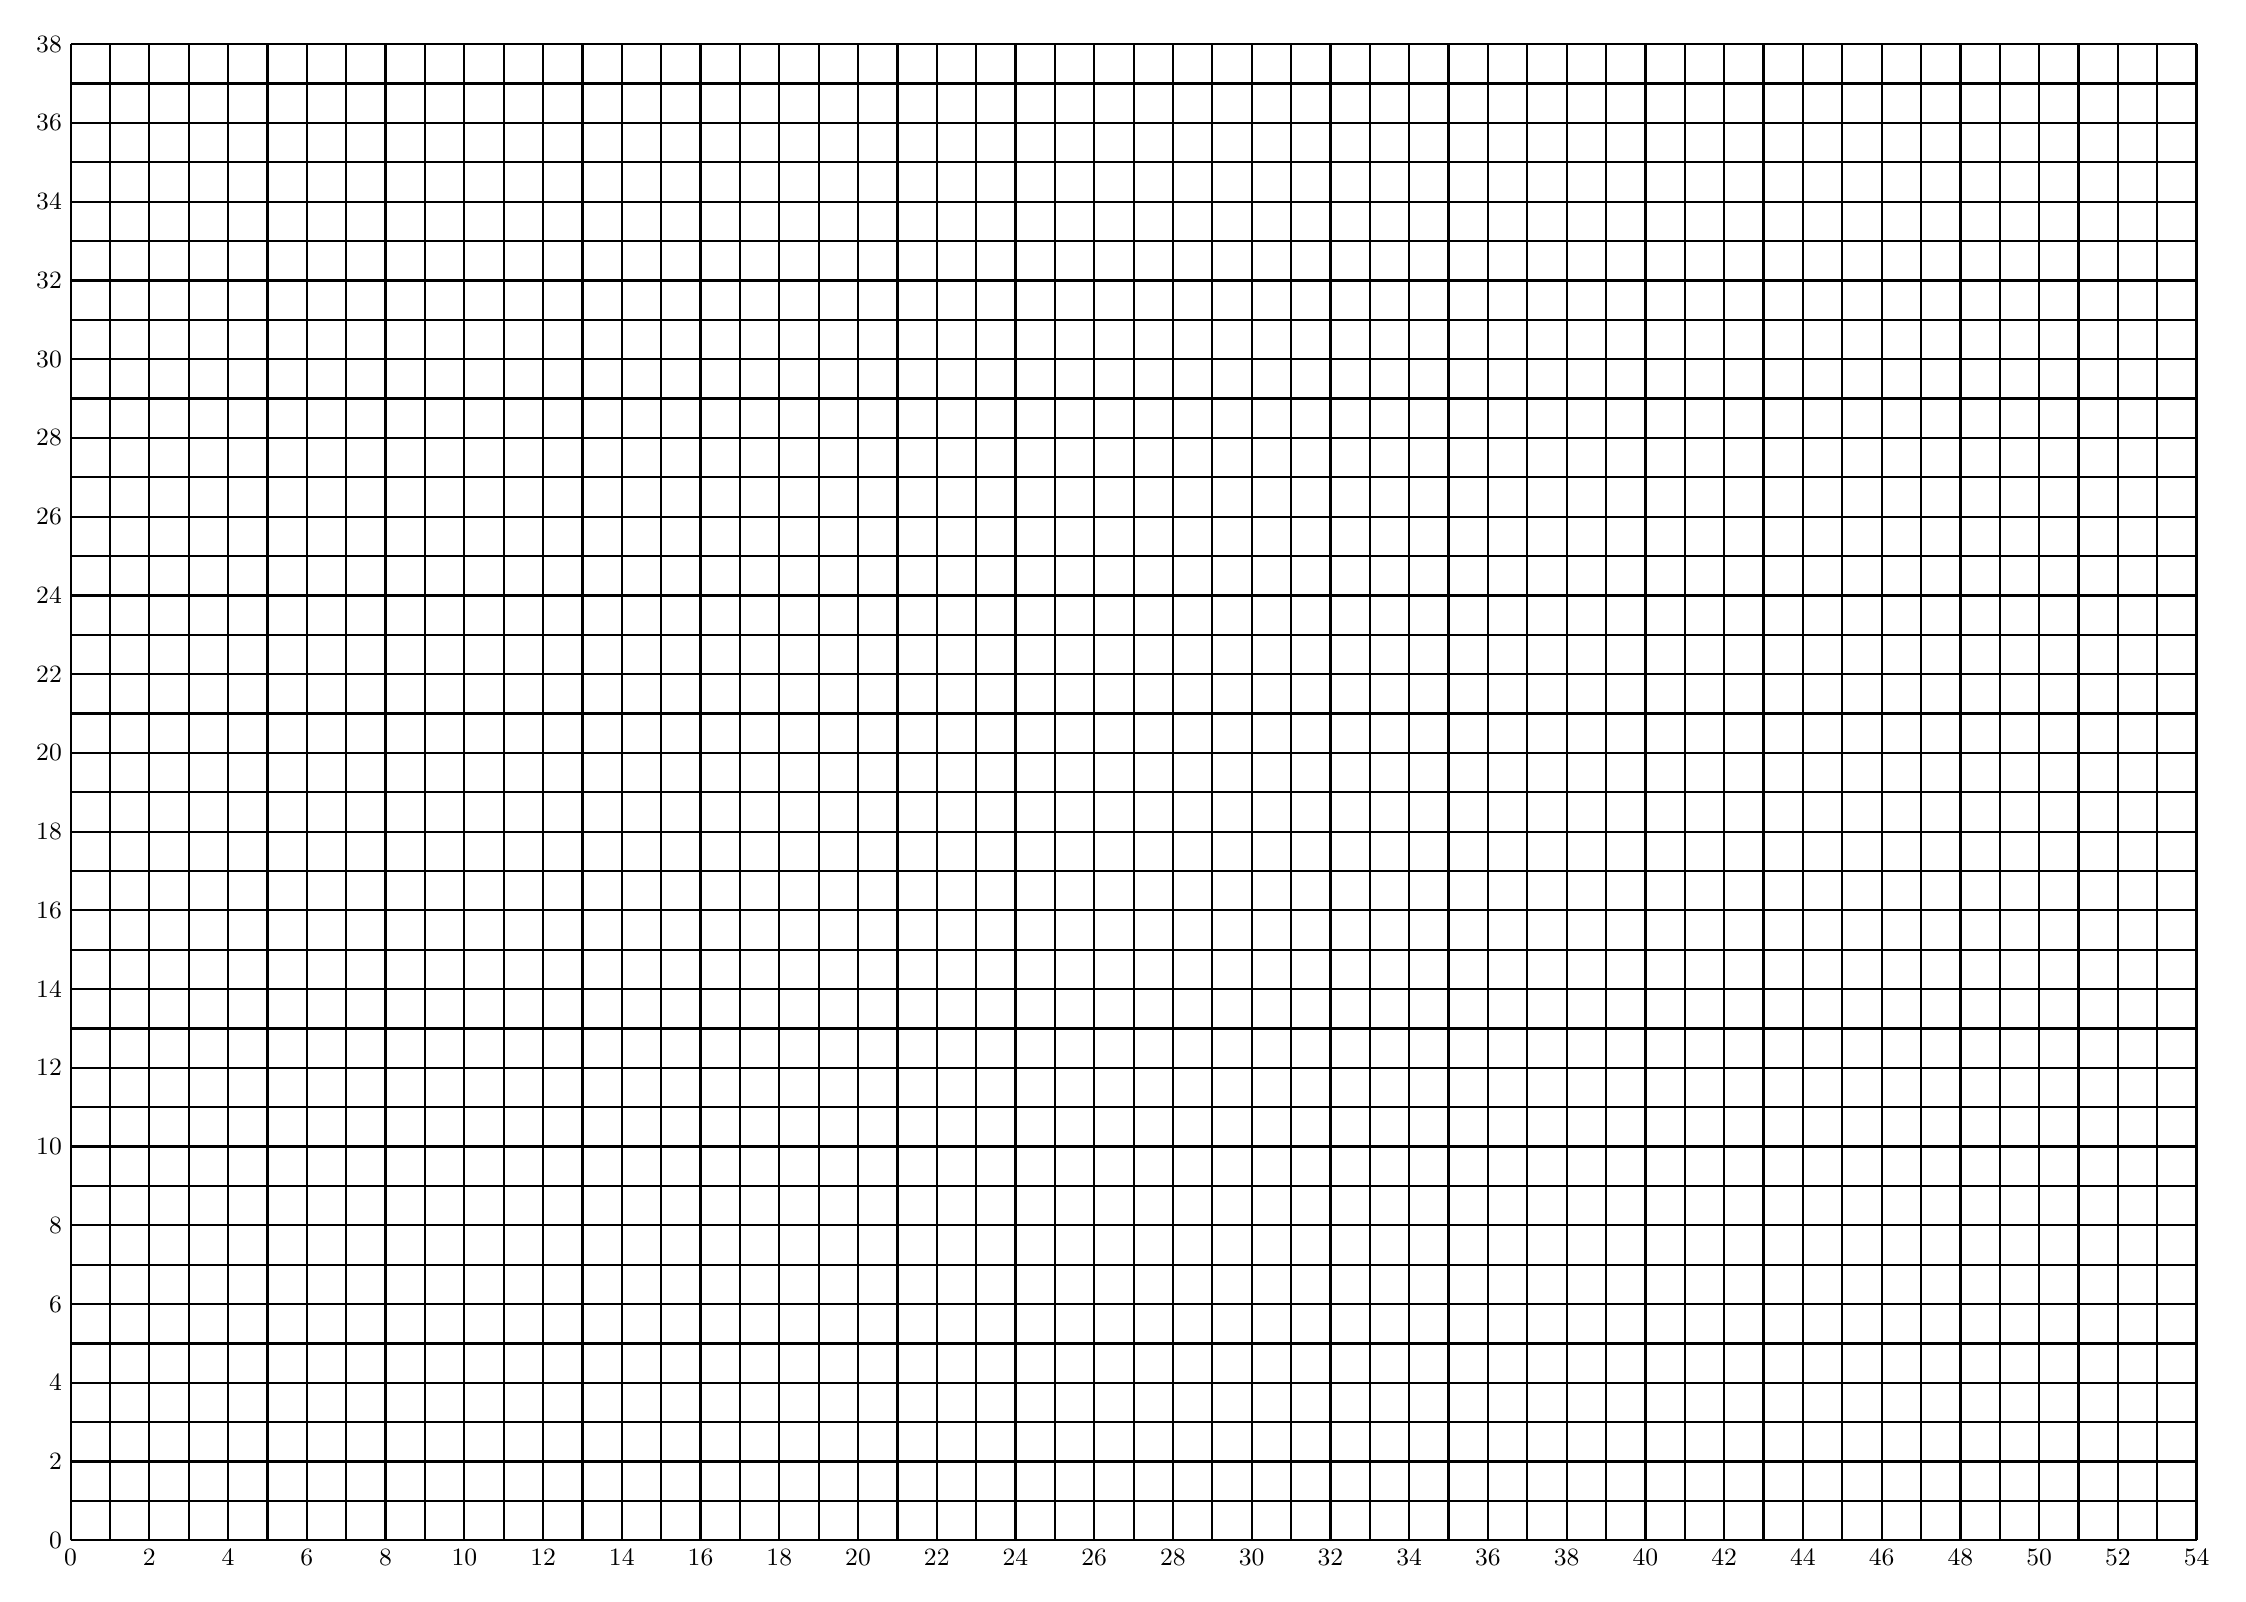
\begin{tikzpicture}
        \foreach \i in {\xMin,...,\xMax} {
            \draw [very thin,black] (\i,\yMin) -- (\i,\yMax)  node [below] at (\i,\yMin) {$\the\numexpr2*\i$};
        }
        \foreach \i in {\yMin,...,\yMax} {
            \draw [very thin,black] (\xMin,\i) -- (\xMax,\i) node [left] at (\xMin,\i) {$\the\numexpr2*\i$};
        }
        \draw [step=1.0,black, thick] (0.0,0.0) grid (27.0,19.0);
        \draw [thick, black, step=1.0cm,xshift=-0.5cm, yshift=-0.5cm] (0.5,0.5) grid +(27.0,19.0);
    \end{tikzpicture}


	% \begin{multicols*}{3}
	% \kactlchapter{appendix}
	% \end{multicols*}
\end{document}
